\newpage
\section*{Git}

Git is a distributed version control system (VCS) that revolutionized the way software projects are managed and collaborated upon. It was created by Linus Torvalds in 2005 to address the scalability and performance limitations of existing VCS tools. In this report, we will delve into the world of Git, examining its key features, benefits, and its impact on modern software development practices.

\subsection*{Key Features of Git}

\begin{enumerate}
    \item Distributed Architecture: Unlike centralized VCS, Git follows a distributed model where each user has a complete local copy of the repository. This allows for offline work, faster operations, and increased resilience.

    \item Branching and Merging: Git's powerful branching and merging capabilities enable parallel development, easy experimentation, and seamless integration of changes. Developers can create branches, work on features independently, and merge their changes back into the main codebase.

    \item Lightweight and Fast: Git is designed to be lightweight, with a small footprint and fast performance. It achieves this through efficient data storage, compression techniques, and optimized algorithms, allowing for swift operations even on large codebases.

    \item Commit History and Tracking: Git provides a detailed commit history, capturing the evolution of the codebase over time. Developers can easily track changes, view commit metadata, and understand the context behind modifications.

    \item Staging Area: Git introduces the concept of a staging area or index, where developers can selectively choose which changes to include in a commit. This granular control allows for more flexible and organized commits.

    \item Distributed Collaboration: Git facilitates seamless collaboration among distributed teams. Developers can share their changes through repositories, clone remote repositories, and synchronize modifications using push and pull operations.
\end{enumerate}

\subsection*{Benefits of Git}
\begin{enumerate}
    \item Scalability: Git's distributed architecture makes it highly scalable, allowing projects of any size to be efficiently managed. The system handles large codebases with ease, making it suitable for both small teams and large enterprise projects.
    \item Speed and Performance: Git's optimized design ensures fast operations, even on complex codebases with extensive histories. This enables developers to work efficiently, reducing wait times and increasing productivity.
    \item Flexibility and Branching Strategies: Git's branching and merging capabilities provide unparalleled flexibility in managing concurrent development efforts. It supports various branching strategies, such as feature branching or release branching, enabling teams to tailor their workflows to project requirements.
    \item Versioning and Rollbacks: Git's version control capabilities allow for easy versioning and rollbacks. Developers can tag specific points in the codebase, create branches for different releases, and revert to previous versions if needed, providing a safety net during software development.
    \item Collaboration and Code Review: Git's distributed nature and support for remote repositories facilitate efficient collaboration. Developers can clone repositories, work on separate branches, review and discuss changes through pull requests, and integrate modifications seamlessly.
\end{enumerate}

\subsection*{Git in Modern Software Development}
\begin{enumerate}
    \item Open Source and Community: Git has gained immense popularity and has become the de facto standard for version control in open-source projects. It has a thriving community, with extensive documentation, online resources, and support from developers worldwide.
    \item Integration and Ecosystem: Git integrates with various development tools, such as integrated development environments (IDEs), continuous integration/continuous delivery (CI/CD) systems, and code review platforms. This integration strengthens the software development ecosystem and streamlines workflows.
    \item Adoption and Industry Impact: Git has had a significant impact on the software development industry, transforming the way teams collaborate, manage code, and track changes. Its popularity and widespread adoption have made it an essential skill for developers and a standard requirement in many software development job roles.
\end{enumerate}

\subsection*{Applications of Git}
Git, as a versatile and widely adopted version control system, finds extensive applications across various areas of software development. Its robust features, distributed architecture, and collaborative capabilities make it a valuable tool for teams of all sizes. In this section, we will explore the diverse applications of Git and how it benefits different aspects of the software development lifecycle.

\begin{enumerate}
    \item \textbf{Source Code Management : }Git's primary application lies in source code management, enabling teams to track, manage, and version their codebase effectively. It offers the following benefits:
    \begin{enumerate}
        \item Version Control: Git tracks changes at a granular level, providing a detailed history of modifications. This enables developers to easily navigate through different versions, review changes, and revert to previous states when needed.
        \item Collaboration: Git allows multiple developers to work on the same codebase concurrently. It enables seamless collaboration by providing mechanisms to merge and synchronize changes, resolve conflicts, and review code through pull requests.
        \item Branching and Parallel Development: Git's branching and merging capabilities facilitate parallel development, where developers can work on separate branches to implement features, bug fixes, or experiments. Branches provide isolation, allowing changes to be developed independently and merged back into the main codebase.
        \item Code Review: Git integrates with code review tools and workflows, enabling teams to perform thorough code reviews. It allows developers to submit changes for review, comment on code, suggest improvements, and ensure code quality before merging it into the main codebase.
    \end{enumerate}
    \item \textbf{Continuous Integration and Deployment (CI/CD) : }Git plays a vital role in CI/CD workflows, ensuring smooth and automated software delivery. Its applications in this area include:
    \begin{enumerate}
        \item Integration with CI/CD Tools: Git seamlessly integrates with CI/CD tools, enabling automated build, test, and deployment processes. CI/CD pipelines can be triggered by code changes, and Git repositories serve as the source of truth for these pipelines.
        \item Automated Testing: Git's versioning capabilities support the creation of automated test suites. Tests can be executed against different versions or branches, ensuring that changes do not introduce regressions and maintaining code quality.
        \item Continuous Deployment: Git, combined with CI/CD practices, allows for continuous deployment of software. It enables automated deployment pipelines that deliver new features or bug fixes to production environments efficiently and reliably.
    \end{enumerate}
    \item \textbf{Project Management and Collaboration : }Git facilitates project management and collaboration, enhancing team productivity and coordination. Its applications in this domain include:
    \begin{enumerate}
        \item 3.1 Task Tracking: Git integrates with project management tools that enable teams to link code changes to specific tasks, issues, or user stories. This helps in tracking progress, associating changes with their corresponding requirements, and maintaining traceability.

        \item Team Collaboration: Git's distributed nature and support for remote repositories enable geographically distributed teams to collaborate effectively. Developers can work on their local copies, share changes through repositories, and synchronize modifications using push and pull operations.

        \item Workflow Customization: Git's flexibility allows teams to define and customize their workflows. They can adopt various branching strategies (e.g., feature branching or GitFlow) and tailor their processes to meet their project's specific needs and requirements.
    \end{enumerate}
    \item \textbf{Open-Source Development : }Git has become the go-to version control system for open-source development, powering numerous collaborative projects. Its applications in the open-source ecosystem include:
    \begin{enumerate}
        \item Code Contribution: Git simplifies the process of contributing code to open-source projects. Developers can fork repositories, make changes in their own branches, and submit pull requests to have their changes reviewed and potentially merged into the main codebase.
        \item Community Collaboration: Git's distributed nature fosters community collaboration and enables developers from around the world to contribute to open-source projects. It facilitates code review, feedback exchange, and knowledge sharing within the open-source community.
        \item Project Forking and Branching: Git allows individuals or teams to create forks of existing projects. Forking enables independent development, experimentation, and customization while maintaining the project's original source as a base. Developers can also create branches within forks to work on specific features or improvements.
    \end{enumerate}
    \item \textbf{Documentation and Content Management : } Git is not limited to code but can also be used for managing documentation, content, and other non-code assets. Its applications in this area include:
    \begin{enumerate}
        \item Versioning and Tracking: Git's version control capabilities extend beyond code, making it suitable for managing documentation, configuration files, and other project assets. It enables tracking changes, reviewing modifications, and maintaining a history of content revisions.

        \item Collaboration: Git's collaborative features facilitate teamwork in documentation and content creation. Multiple contributors can work on different branches, review and comment on changes, and merge updates to create a cohesive and up-to-date final product.

        \item Content Publishing: Git can be used for publishing content, such as websites or documentation sites, by leveraging Git-based publishing platforms. It allows for easy deployment of changes, ensuring that published content reflects the latest updates from the Git repository.
    \end{enumerate}
    \item Git's versatility and powerful features make it indispensable in various applications within the software development lifecycle. From source code management to collaboration, CI/CD workflows, project management, open-source development, and content management, Git provides the foundation for efficient and collaborative software development. Its distributed architecture, branching capabilities, and seamless integration with development tools have positioned Git as a standard and widely adopted version control system in the industry.
\end{enumerate}


Git has revolutionized the world of version control systems with its distributed architecture, powerful branching capabilities, speed, and flexibility. Its benefits, such as scalability, collaboration support, and efficient code management, have made it a cornerstone of modern software development practices. Git's impact on the industry and its widespread adoption underline its significance in empowering developers to work effectively, collaborate seamlessly, and manage codebase versions with ease.

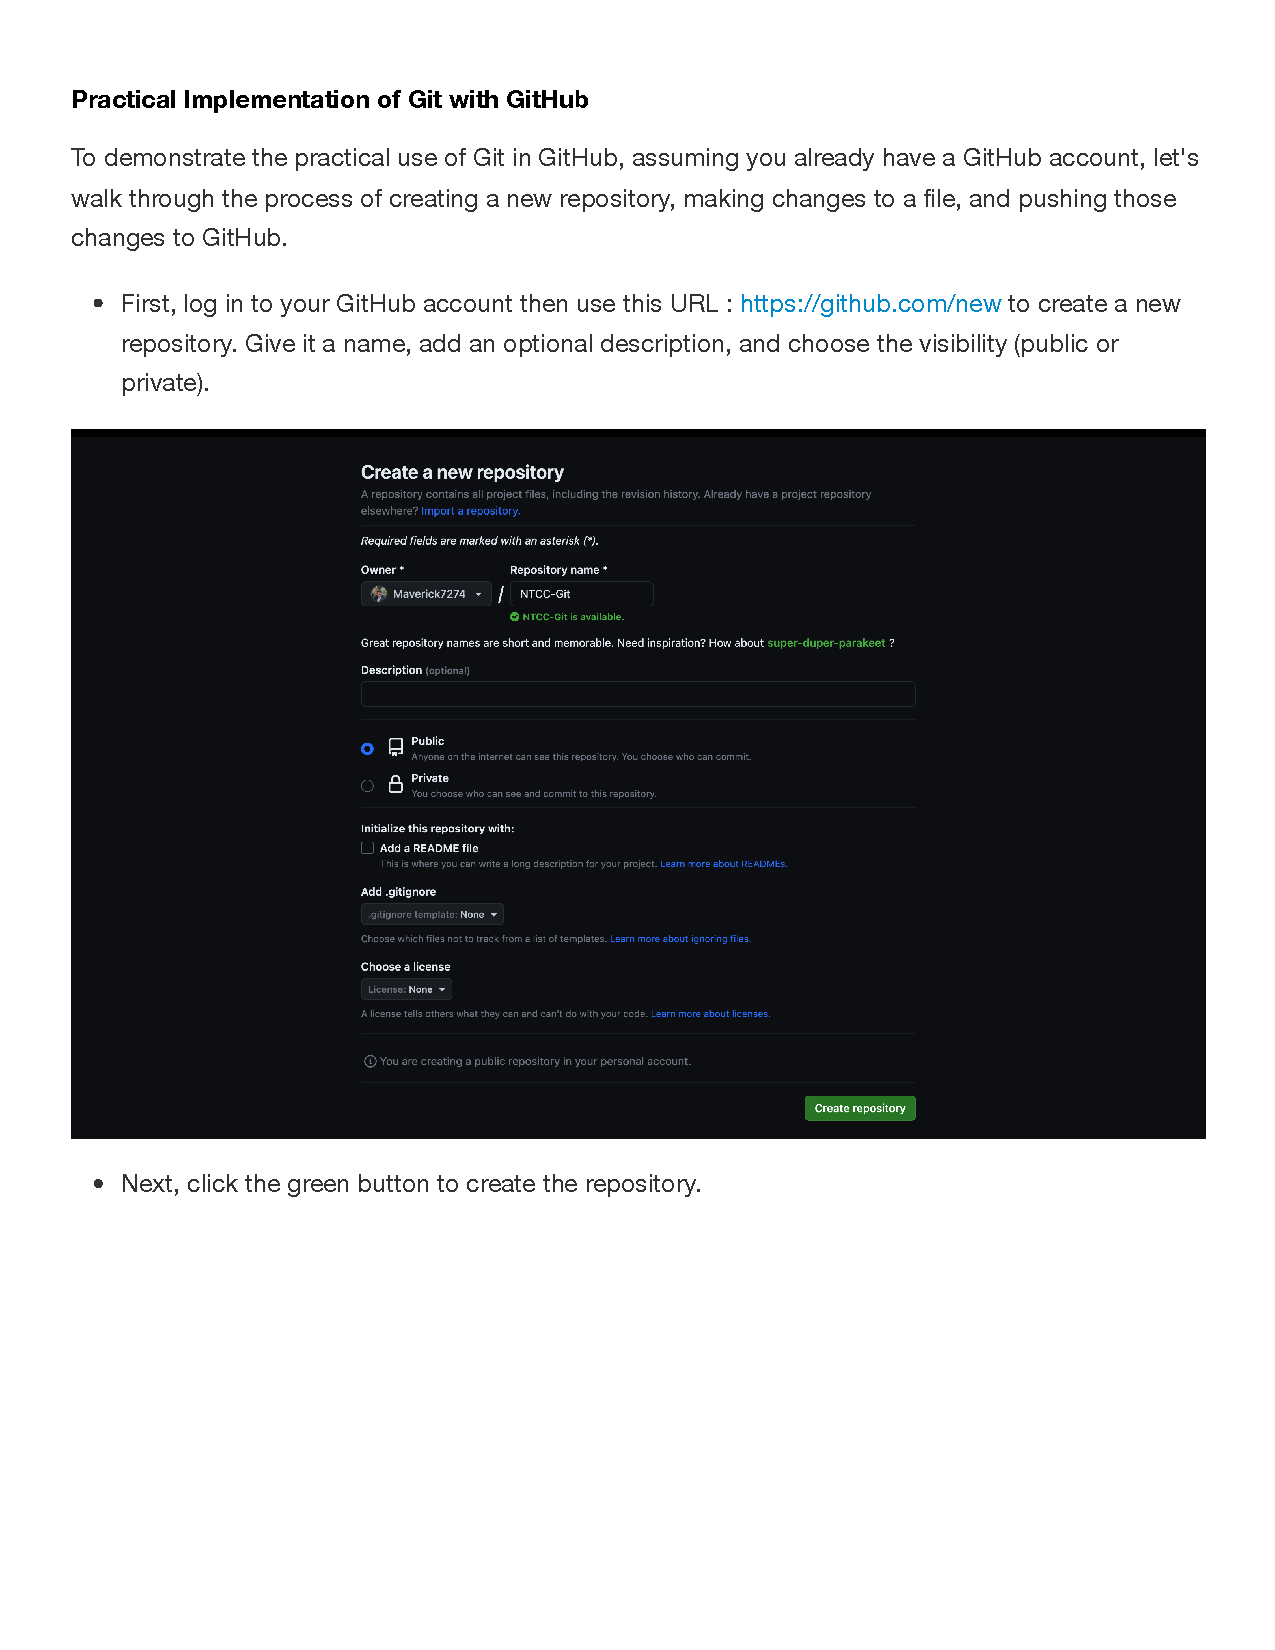
\includepdf[pages=-]{Assets/git.pdf}